\newtheoremstyle{break}{\baselineskip}{0.5\baselineskip}{\itshape}{}{\bfseries}{}{\newline}{}

\theoremstyle{break}
\newtheorem{thm}{Theorem}[section]
\newtheorem{cor}[thm]{Corollary}
\newtheorem{lem}[thm]{Lemma}
%\theoremstyle{definition}
\newtheorem{defin}[thm]{Definition}

\lstset{ %
basicstyle=\footnotesize,       % the size of the fonts that are used for the code
numbers=left,                   % where to put the line-numbers
numberstyle=\footnotesize,      % the size of the fonts that are used for the line-numbers
stepnumber=2,                   % the step between two line-numbers. If it's 1 each line will be numbered
numbersep=5pt,                  % how far the line-numbers are from the code
backgroundcolor=\color{white},  % choose the background color. You must add \usepackage{color}
showspaces=false,               % show spaces adding particular underscores
showstringspaces=false,         % underline spaces within strings
showtabs=false,                 % show tabs within strings adding particular underscores
frame=single,			% adds a frame around the code
tabsize=2,			% sets default tabsize to 2 spaces
captionpos=b,			% sets the caption-position to bottom
breaklines=true,		% sets automatic line breaking
breakatwhitespace=false,	% sets if automatic breaks should only happen at whitespace
escapeinside={\%*}{*)}          % if you want to add a comment within your code
}

\addbibresource{report.bib}

\DeclareGraphicsExtensions{.pdf,.png}
\dominitoc

% Define bijection symbol as defined in the oz package.
% We cannot include the oz package directly because of double definitions. This is a work-around.
\let \tfun \rightarrow
\let \tinj \rightarrowtail
\def \bij {\mathrel{\ooalign{$\tinj$\hfil\cr$\mkern5mu\tfun$}}}

\DeclareMathSymbol{\mstar}{\mathord}{symbols}{"03}
\DeclareMathOperator{\sat}{sat}
\DeclareMathOperator{\new}{\mathbf{new}}
\DeclareMathOperator{\prefix}{\#}
\DeclareMathOperator{\append}{@\:}
\newcommand\type[1]{\mathsf{#1}}

\newcommand\isabelleref[2]{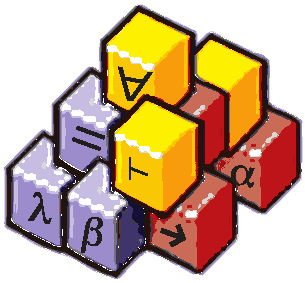
\includegraphics[height=0.75\baselineskip,keepaspectratio]{images/isabelle_logo.pdf} \texttt{\detokenize{#1}} in \texttt{\detokenize{#2}}}
\newcommand\isabellelref[2]{\begin{flushright}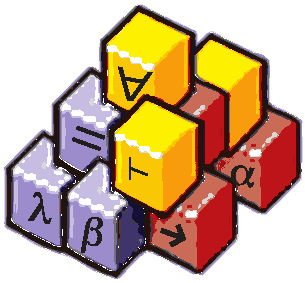
\includegraphics[height=0.75\baselineskip,keepaspectratio]{images/isabelle_logo.pdf} Also see \emph{\texttt{\detokenize{#1}}} in \emph{\texttt{\detokenize{#2}}}\end{flushright}}

\usetikzlibrary{arrows.meta}
\tikzstyle{data}=[rectangle split,rectangle split parts=2,draw,text centered]

\isabellestyle{it}
%\bibliographystyle{acm}

% Custom todo commands
\newcommand\writingtask[1]{\todo[inline]{\textbf{Writing task}: #1}}
\newcommand\missingref[1]{\todo[inline, inlinewidth=2.1cm, noinlinepar, nolist, color=gray!40, size=\tiny]{Missing reference}\todo[color=gray!40, caption={\textbf{Reference missing}: #1}]{#1}}
\newcommand\spellcheck[1]{\todo[color=green!70]{\textbf{Grammar and spellcheck}: #1}}
\newcommand\feedback[1]{\todo[color=blue!70]{\textbf{Proposed feedback}: #1}}